The Robot Control Testbed (RCT) is a collection of robot--based applications
under development in the research group ASLab. The robots include commenrcial
research platforms, simulated robotos and custom mobile robot
implementations. 

Higgs is a custom robot that is part of thr RTC developments. This is a mobile
robotic system which consists of a base platform and different interconnected
subsystems to cover a wide range of capabilities. The research aim is to
provide the mobile robot with the necessary cognitive capabilities and an
intelligent control system, as to perform complex tasks. 

This manual includes information concerning its software and
hardware description, specification, and use cases and additional information.
 The following sections summarise the key aspects of the testbed.

\section{Higgs Structural Description}

\subsection{Base Platform}
The base platform of Higgs is a mobile robot Pioneer 2--AT8 which has been
designed by ActivMedia Robotics (Fig. \ref{Higgs}). It is a robust platform which includes all the necessary elements to implement a control and navigating system, specially designed for outdoor applications.  Additional systems and elements can be attached to this platform. The base platform is given the ASLab name Higgs, as a reference to the Higgs' bosson.\\
 
\begin{figure}[htdp]
\begin{center}
 {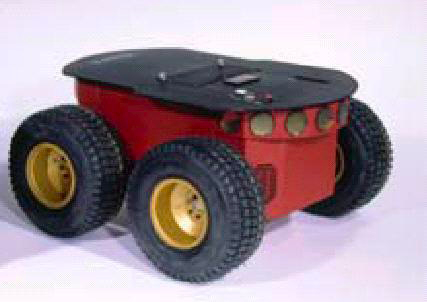
\includegraphics[width=0.75\textwidth]{Higgs.jpg}}
\end{center}
\caption{The Pioneer 2-AT8 platform used to implement the RCT Higgs robot.}
\label{Higgs}
\end{figure}


Higgs is a small size mobile robot, with a support structure made of aluminium. Its total weight is of 15 kg, being capable of carrying up to 40 kg. From a hardware viewpoint, the mobile robot consists of different elements: 

%AUG 2009 BE AWARE: each subsystem or element should have both an structural and a functional brief description!!
\begin{description}
\item Robot Panel: it is the superior platform of the robot, designed for a later assembly of new elements such as cameras or laser systems. 
\item Robot Body: it is a box--shaped element made of aluminium. It contains the batteries, the actuators, the electronic circuits and the rest of elements. It also allows to attach additional elements such as an onboard PC, a modem or additional sensors.
\item Control Panel: it is the access panel to the robot's microcontroller, placed in the robot panel. It consists of several control buttons, robot status leds (robot switch on, microcontroller status, battery charge) and a serial port RS--232 to be used as an input and output communication link with a external PC.
\item Sensors: the mobile robot is provided with two arrays of eight sensors each, which allow the detection and location of objects in the mobile robot environment. The arrays are placed at the front and at the rear part of the robot.
\item Actuators: the robots contains 4 Pittman motors GM9236E204. Each one includes an optical encoder to determine the robot's speed and position. 
\item Microcontroller: it is a Hitachi H8S microcontroller consisting of different elements (memories, serial ports, inputs, outputs, 8 bit bus) which carries out different operations such as trigger and register the sensors' signal, control the actuators, and some other low--level operations.
\item Bumpers: they are additional elements attached to the platform, 5 at the front and 5 at the rear.
\item Power: there are three batteries 12 VDC 7 Ah--h, located at the rear part of the robot. They provide 252 W--h, which assure several hours of autonomy movement to the robot. Their status can be checked in the corresponding led of the control panel.
\end{description}

% From HiggsManual. There is much more than the things written here
In addition to the hardware, the mobile robot has different software elements, either provided by the manufacturer or developed by ASLab team members. 
\begin{description}
\item AROS (ActivMedia Robotics Operating System): it is the operating system, consisting in server processes running on the Hitachi microcontroller in Higgs. It is a low--level software in charge of regulating the motors' speed, sonars' signal, encoders' signal and other low--level tasks. This software will also communicate the obtained information to other client software applications through the RS-232 serial interface.
\item ARIA: it is an applications--programming interface (API) based on C++ to control the robot. It acts as the client in the client--server topology. It allows to program high--level software applications, such as intelligent behaviour (obstacle avoidance, object recognition, wandering, exploration, etc). The robot control is based on direct commands, movement commands or abstract--level actions.
\item ASLab team software: there are a set of modules developed by the ASLab team members to extend or to add capabilities of Higgs. The modules developed are: communication \cite{Pareja2004}, synthetic emotions \cite{Conde2005}, SOAR integration \cite{Sanchez2005}, voice \cite{Panizo2005}, RT--CORBA control server \cite{Hernando2005}, RT--CORBA robot status register, Java based CORBA client, CORBA based remote operation \cite{Conejo2007}, and surface recognition \cite{Godoy2007}. 
\end{description}

%some of the last devices not included in Manual Higgs, so not much info!!
\subsection{Onboard Systems}

On the base platform, different devices have been attached to expand the original range of functionalities of the mobile robot (Fig. \ref{higgswithonboarddevices}).\\

\begin{figure}[htdp]
\begin{center}
 {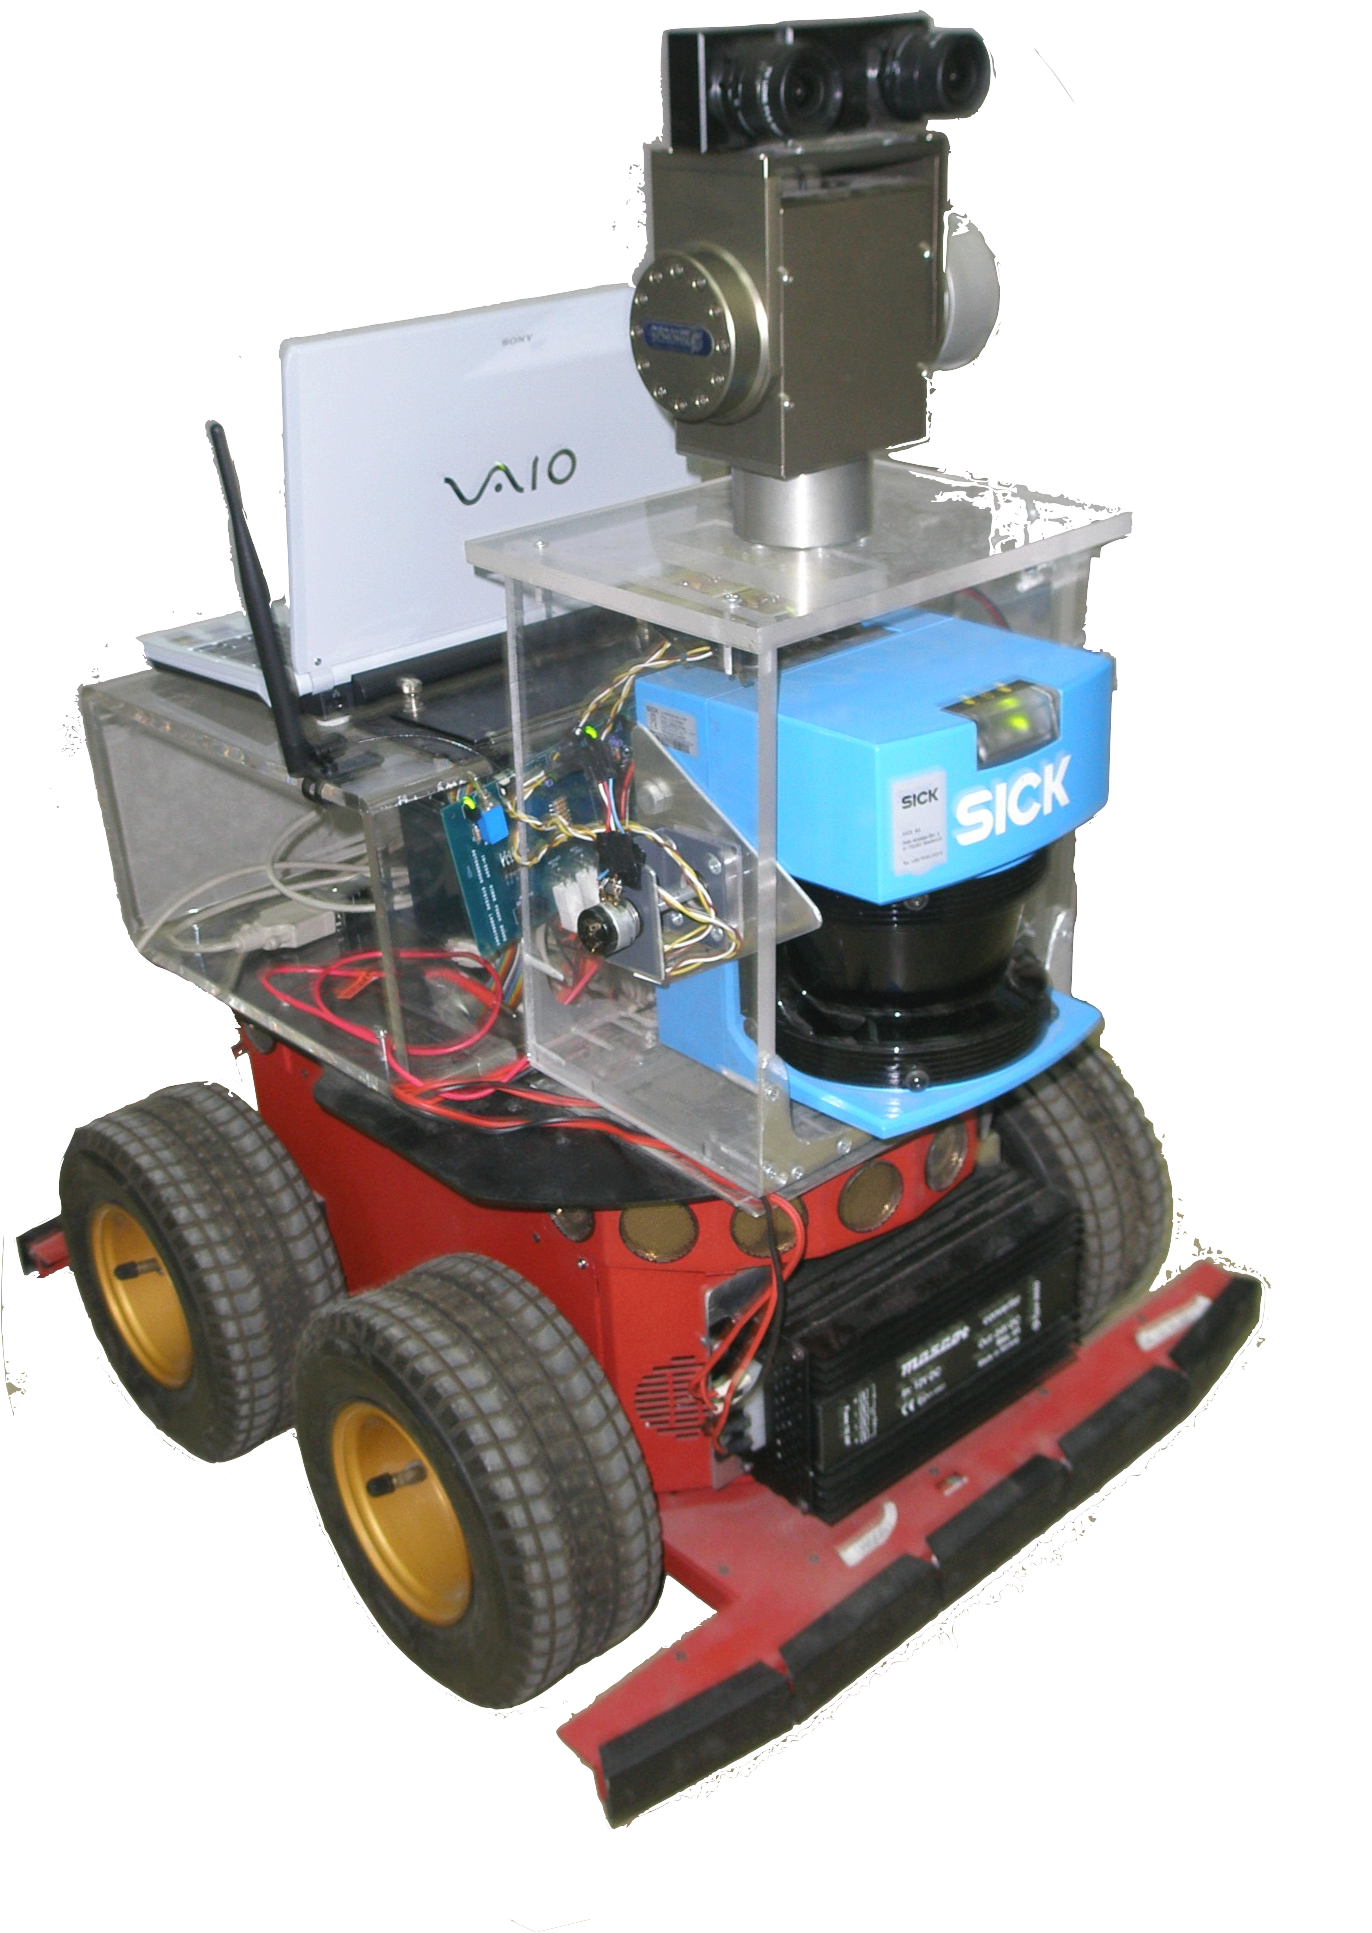
\includegraphics[width=0.65\textwidth]{higgs.png}}
\end{center}
\caption{Pioneer 2-AT8 (Higgs) with onboard systems}
\label{higgswithonboarddevices}
\end{figure}

\begin{itemize}
\item Onboard Computer:  it is a computer attached to the base platform whose mission is to facilitate the communication with the microcontroller, the control of the robot, the execution of complex navigation operations, and additional communication operations. Taking into consideration several requirements and operational constraints defined in \cite{ManualHiggs}, a GENE--6330 was chosen. Related to software, the onboard computer uses Linux as operating system, as well as having a real--time software RTAI and RT--CORBA server.
\item Laser: it is a laser scanner for mobile robotics applications, placed at the front part of the robot panel.
\item Wrist: it is a 2 DOF high precision and torque actuator for orientation of the camera. It is attached to the laser.
\item Camera: it is a stereo camera that will be used as the robot's vision system, attached to the wrist.
\item Radio: it is a radio system for DGPS.
\item Laptop: it is a lightweight high functional laptop.
\item GPS: it is a high performance GPS system.
\end{itemize}

\subsection{Supporting Systems} 
Along with the base platform and the onboard systems, Higgs includes some
additional supporting systems to complete its functioning.

\begin{enumerate}
\item Wireless Network: it is an additional subsystem included in the testbed to allow the communication with the wireless local network in the ASLab laboratory. It consists of a wireless card (placed in the onboard computer), an antenna necessary as the wireless card is placed inside the aluminium robot body (attached to the robot panel), and an access point (connected to the laboratory LAN).
\item Remote Control: it is a portable device to remote control the robot.
\item Server
\item User Terminal
\end{enumerate}

\section{Robot Functional Description}

The functional description of the Higgs robot Testbed has been made
through the specification of use cases and requirements (see Chapter
\ref{chapter:asyshiggs}). \emph{FunctionalRequirement} has been defined in the
ontology as a requirement that specifies an operation or behaviour a system must perform.\\

For the RCT, the functional requirements considered can be classified into primary  and secondary ones. A primary functional requirement refers to a main capability to be fulfilled by the system. In the case of the RCT, two primary functional requirements have been considered: navigation, and survival. \\

A secondary functional requirement refers to an additional capability desired in the system. For the RCT, these secondary functional requirements are: to explore the environment, to avoid an obstacle while moving or exploring, reactive movement, the identification of an object in the environment, and search. Some additional functional requirements expand or detail the former ones, such as autonomous navigation as an extended case of the navigation one.\\

